\chapter{Fundamentação Teórica}
\label{chap:fundamentacaoTeorica}


Para entendermos o porquê de utilizar mais de um banco de dados em uma mesma aplicação, temos que entender o que é um banco de dados, quais gêneros existem e em qual tipo de problema cada gênero se destaca.

Este capítulo está organizado em duas seções, a \autoref{sec:database} apresenta o conceito de banco de dados. Já a \autoref{sec:databasetype} apresenta os gêneros de bancos de dados mais utilizados atualmente e constrasta o conceito dos modelos relacional e não-relacional. Ainda nessa seção é apresentada a definição de persistência poliglota.

\section{Banco de Dados}
\label{sec:database}

Banco de dados é um sistema computadorizado de manutenção de registros, análogo à um armário de arquivamento eletrônico. Podemos entendê-lo como um repositório para manter uma coleção de arquivos de dados computadorizados \cite{CJDate}. \citeonline{Elmasri} define banco de dados como uma coleção de dados relacionados e que dados são fatos com um significado implícito. Porém, a definição de \citeonline{Elmasri} é mais abrangente, logo ele aponta três propriedades implícitas para restringir a definição de banco de dados.

A primeira propriedade é que um banco de dados deve representar alguns aspectos do mundo real, chamado de \textit{\ac{UoD}}. As alterações que ocorrem nesse universo são refletidas em um banco de dados. A segunda propriedade define que o banco de dados é uma coleção lógica e coerente de dados com algum significado inerente, ou seja, uma coleção de dados randômicos não pode ser considerado um banco de dados. A terceira propriedade afirma que banco de dados é projetado, construído e povoado com dados, atendendo a uma proposta específica. Além disso, possui um grupo de usuários definido e algumas aplicações preconcebidas, de acordo com o interesse desse grupo.

Os bancos de dados têm contribuído para o aumento do uso do computador \cite{Elmasri} e podemos afirmar que eles apresentam um papel crucial em quase todas as áreas em que os computadores são utilizados. Em consequência, o estudo sobre banco de dados é extremamente necessário para os profissionais da computação.

Antes da existência dos bancos de dados, a aplicação devia gerenciar e processar arquivos para manter os dados persistidos. Para justificar o uso de banco de dados, \citeonline{Elmasri} cita quatro características: natureza autodescritiva, abstração de dados, suporte para as múltiplas visões de dados e processamento de transações de múltiplos usuários.

A primeira característica, \textbf{natureza autodescritiva do banco de dados}, apresenta o catálogo do banco de dados como uma grande vantagem sobre o processamento tradicional dos arquivos, pois o catálogo identifica as estruturas dos arquivos, formato e tipo de dados. Logo, não é necessário conhecer a aplicação para trabalhar com os dados. Já  o processamento tradicional dos arquivos, mantém essas definições de estrutura na própria aplicação \cite{Elmasri}.

Em relação à característica \textbf{abstração de dados}, \citeonline{Elmasri} afirma que não é feita no processamento tradicional de arquivos, pois é a aplicação que define a estrutura dos dados. Por exemplo, suponha que tenhamos diversos programas utilizando o mesmo arquivo para armazenar uma coleção de dados. Se um desses programas precisar de acrescentar algum campo novo, todos os outros programas que acessam esse arquivo, devem ser modificados para contemplar o novo campo adicionado. Já quando utilizamos banco de dados, a alteração da estrutura dos dados pode não influenciar no funcionamento dos outros programas.

Em relação à característica \textbf{suporte para múltiplas visões dos dados}, \citeonline{Elmasri} diz que quando é utilizado o banco de dados, é possível ter diferentes visões sobre os dados, fazendo o cruzamento das tabelas. Com a abordagem de processamento de arquivo tradicional, isso não é usual.

A última característica citada por \citeonline{Elmasri} é o \textbf{processamento de transações de múltiplos usuários}, essa característica é essencial para que várias aplicações possam acessar e alterar os dados a partir de usuários diferentes e simultâneos. Porém, o \ac{SGBD} deve ter implementado um controle de concorrência para garantir a atomicidade das transações e a consistência dos mesmos dados.

\citeonline{Elmasri} não cita a existência dos bancos de dados NoSQL, que são bancos que não têm esquema pré-definido, chamados de \textit{schemaless}. Apesar de não ter a declaração do tipo de estruturas de dados contidas no banco, os bancos de dados \textit{schemaless} fazem a abstração dos dados da mesma maneira que os bancos de dados tradicionais, têm suporte para múltiplas visões e múltiplos usuários.

Como revelado acima, a utilização do banco de dados facilita o desenvolvimento das aplicações, permite a abstração entre aplicação e dados e, além disso, faz o controle de concorrência. Após verificarmos que o uso de banco de dados é imprescindível para implementação, deparamo-nos com uma outra dificuldade, qual banco de dados utilizar. 

Os bancos de dados, chamados de NoSQL, chamam a atenção da comunidade científica, depois da publicação de dois artigos BigTable \cite{bigtable} e Dynamo \cite{dynamo}. Essas publicações apresentam bancos de dados NoSQL que têm um desempenho superior ao modelo relacional. O BigTable apresenta um banco de dados orientado a coluna e o Dynamo apresenta um banco de dados chave-valor.

\section{Gêneros de Banco de dados}
\label{sec:databasetype}
Durante anos, o banco de dados relacional tem sido considerado a melhor opção para a maioria dos problemas de persistência. No entanto, o aumento do volume de dados fez com que os especialistas buscassem novas soluções, que permitissem o armazenamento paralelo dos dados, pois o modelo relacional não foi desenhado para funcionar em ambiente distribuído. Logo, os bancos de dados NoSQL se destacaram por funcionarem bem nesse ambiente e terem um melhor desempenho com grande volume de dados \cite{NoSQL}.

Os bancos de dados NoSQL têm as seguintes características: não usam o modelo relacional, foram desenhados para funcionar em ambientes distribuídos, a maioria deles são \textit{open source} e não tem catálogos (\textit{schemaless}) \cite{NoSQL}. Carlo Strozzi foi o primeiro a utilizar o nome NoSQL, mas não no sentido que a palavra tem hoje. Strozzi denominou um banco de dados relacional, \textit{open source} de NoSQL, pois não usava \ac{SQL} como linguagem de consulta. O sentido, que a palavra tem hoje, veio de uma conferência realizada em São Francisco nos Estados Unidos, em Junho de 2009. Johan Oskarsson que organizou essa conferência, escolheu esse nome, porque era uma boa \textit{hashtag} no Twitter, pois era pequeno, memorável e tinha poucos resultados no Google. Isso facilitaria os interessados a encontrar a conferência. Apesar do termo não significar explicitamente o que são esses bancos de dados, atendeu bem a intenção de Oskarsson \cite{NoSQL}.


\subsection{Banco de Dados relacional}
\label{subsec:relationaldatabasetype}
O modelo relacional armazena os dados em tabelas de duas dimensões em linhas e colunas. A interação com esse banco é feita por um \ac{SGBD} que utiliza a \ac{SQL} como linguagem de consulta de dados. Os dados armazenados são valores tipados e podem ser numéricos, texto, data e outros tipos, que são configurados pelo sistema. É possível fazer junção das tabelas e obter diferentes perspectivas das informações de maneira simples. MySQL, Oracle e PostgreSQL são alguns exemplos de banco de dados relacional \cite{SDSW}.
A representação do modelo relacional pode ser feita com o diagrama \ac{UML}. Por exemplo, um sistema de \textit{e-commerce} poderia ser desenhado conforme o diagrama da \autoref{fig:diagrama_sql_uml} e as tuplas ficariam dispostas conforme \autoref{fig:disposicao_tabela}.
\begin{figure}[H]
    \centering
    \caption{Exemplo de um diagrama \ac{UML} para o modelo relacional}
    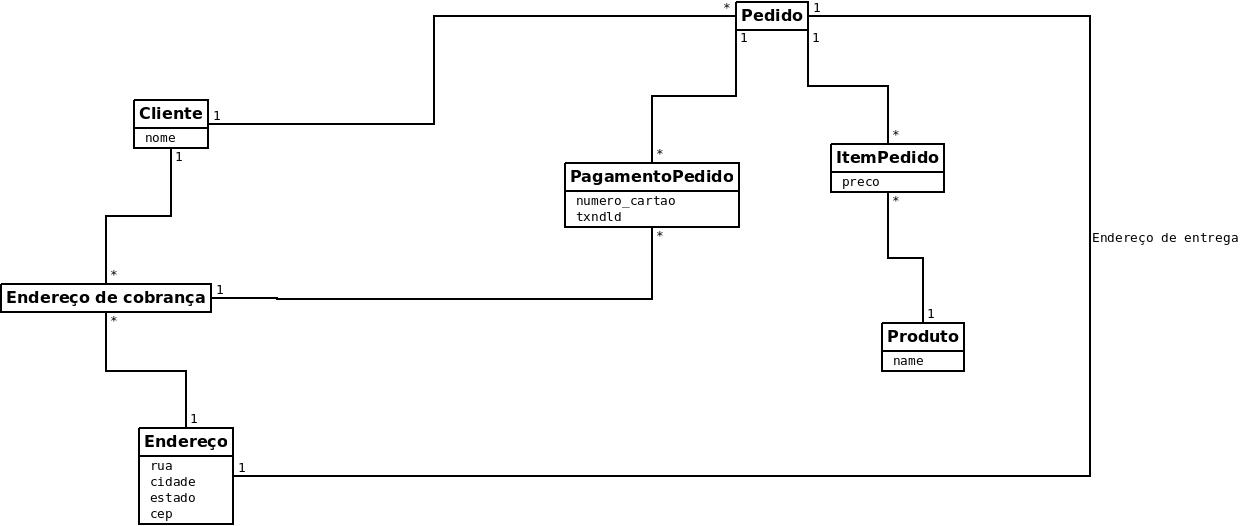
\includegraphics[width=0.8\textwidth]{./04-figuras/diagrama_sql_uml.jpg}
    \fonte{\cite{NoSQL}}
    \label{fig:diagrama_sql_uml}
\end{figure}
\begin{figure}[H]
    \centering
    \caption{Exemplo da disposição dos dados no modelo relacional}
    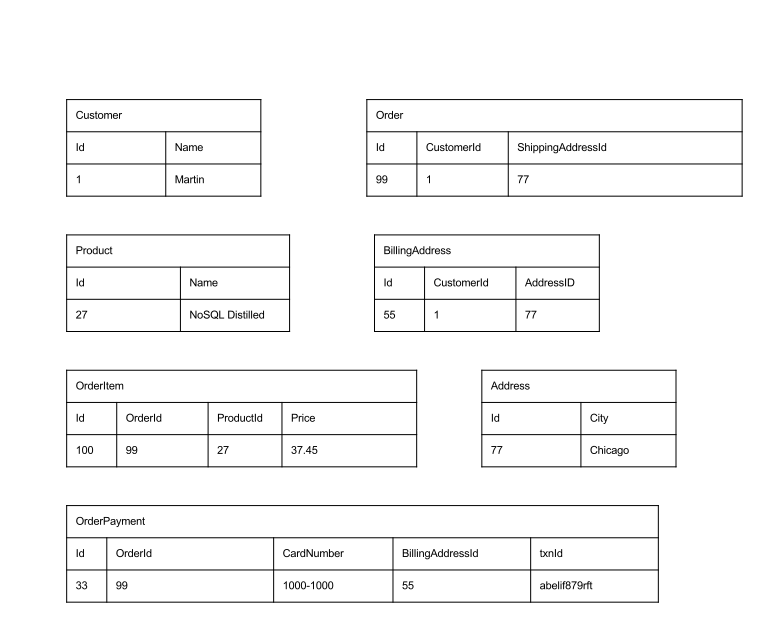
\includegraphics[width=0.8\textwidth]{./04-figuras/disposicao_dados_tabela.png}
    \fonte{\cite{NoSQL}}
    \label{fig:disposicao_tabela}
\end{figure}


O modelo relacional funciona muito bem para diversas aplicações, pois é bem flexível em relação às consultas, permite concorrência, transações e pode ser integrado com várias aplicações. Porém, há uma desvantagem que causa frustação em muitos desenvolvedores, chamada de Impedância de Correspondência ou \textit{Impedance Mismatch} \cite{Elmasri,NoSQL}. Isso ocorre, pois nem sempre o tipo do campo no banco de dados irá corresponder ao tipo esperado da linguagem utilizada, então é necessário criar uma forma de associação entre o tipo da variável da linguagem com o tipo do valor da tabela. Outra desvantagem é que esse não aceita valores multivalorados, distanciando a aplicação ainda mais do modelo relacional.


\subsection{Banco de dados não-relacional}
\label{subsec:nosqldatabasetype}
Os bancos de dados NoSQL foram construídos para suprir a necessidade de se trabalhar com grande quantidade de dados e em \textit{clusters}. NoSQL abrange diversos gêneros de banco de dados, entre eles o orientado a documento, chave-valor, orientado a coluna e orientado a nó.

Todos esses gêneros não possuem catálogo, ou seja, não se define previamente em qual estrutura os dados serão armazenados. Isso permite a criação de sistemas flexíveis, pois a estrutura dos dados pode ser alterada facilmente. É possível adicionar um novo campo, sem ter que se preocupar com a atualização da base legada, pois os objetos de uma mesma coleção podem ter diferentes campos. Da mesma maneira, para descontinuar um campo, basta parar de armazená-lo. Os registros antigos, que tinham esse campo, continuarão com eles e os objetos novos não irão armazená-lo, que já não faz parte da aplicação \cite{NoSQL}.

Com isso é possível trabalhar com dados não uniformes, isto é, campos diferentes para cada registro. Para que o banco de dados relacional lide com um objeto dessa natureza, é necessário uma tabela com os campos de todos os objetos e consequentemente, o banco armazenaria espaços vazios para os campos que não foram preenchidos pelo registro.

Basicamente, os bancos de dados NoSQL deslocam a definição do esquema para a aplicação que acessa o banco. Isso pode se tornar problemático quando há muitas aplicações acessando o mesmo banco, mas existem soluções para resolver isso, uma delas é encapsular toda a interação com o banco de dados, fazendo esse funcionar como um \textit{web service} \cite{NoSQL}.

Além dessa flexibilidade, a maioria dos gêneros NoSQL permite estruturar dados multivalorados\footnote{O banco de dados orientado a nó, é um dos gêneros que não implementam agregação.}. Esses dados são modelados como agregação, que é uma coleção de objetos relacionados que desejamos tratar como um único objeto \cite{domain-driven}. A agregação facilita a manipulação e a consistência desses dados, pois são tratados como uma unidade, ou seja, são lidos e escritos como um conjunto de dados único. Como, geralmente, ao utilizar esse relacionamento buscamos, operações atômicas, essa abordagem se adapta perfeitamente com a aplicação \cite{NoSQL}. Para exemplificar, iremos modelar o exemplo de
\textit{e-commerce} anterior de duas maneiras diferentes.

Na primeira iremos utilizar agregação entre as relações de \textit{Pedido-Endereço}, \textit{Pedido-ItemPedido}, \textit{Pedido-Pagamento}, \textit{Cliente-Endereço}, e por fim \textit{Endereço-Pagamento}. No diagrama, iremos utilizar o símbolo de composição em \ac{UML} para demonstrar como a informação se adapta na estrutura de agregação \cite{NoSQL}.O diagrama ficaria como na \autoref{fig:diagrama_no_sql_uml_simples} e a disposição de dados ficaria como na \autoref{fig:disposicao_json_simples}, a qual utiliza o padrão JSON\footnote{JSON é um tipo de formato e transmissão de dados muito utilizado em JavaScript que representa os dados estruturados de uma maneira simples para as pessoas lerem e escreverem e para as máquinas fazerem a conversão.}.

\begin{figure}[H]
    \centering
    \caption{Exemplo de um diagrama \ac{UML} utilizando agregação}
    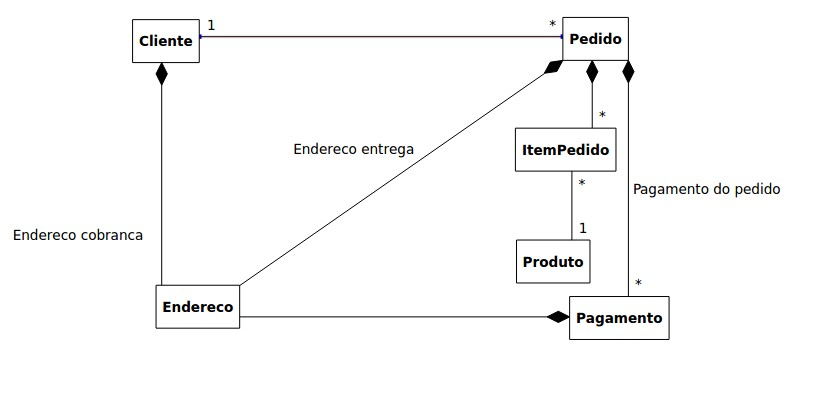
\includegraphics[width=0.8\textwidth]{./04-figuras/diagrama_no_sql_uml_simples.jpg}
    \fonte{\cite{NoSQL}}
    \label{fig:diagrama_no_sql_uml_simples}
\end{figure}
\begin{figure}[H]
    \centering
    \caption{Exemplo da disposição dos dados utilizando agregação}
    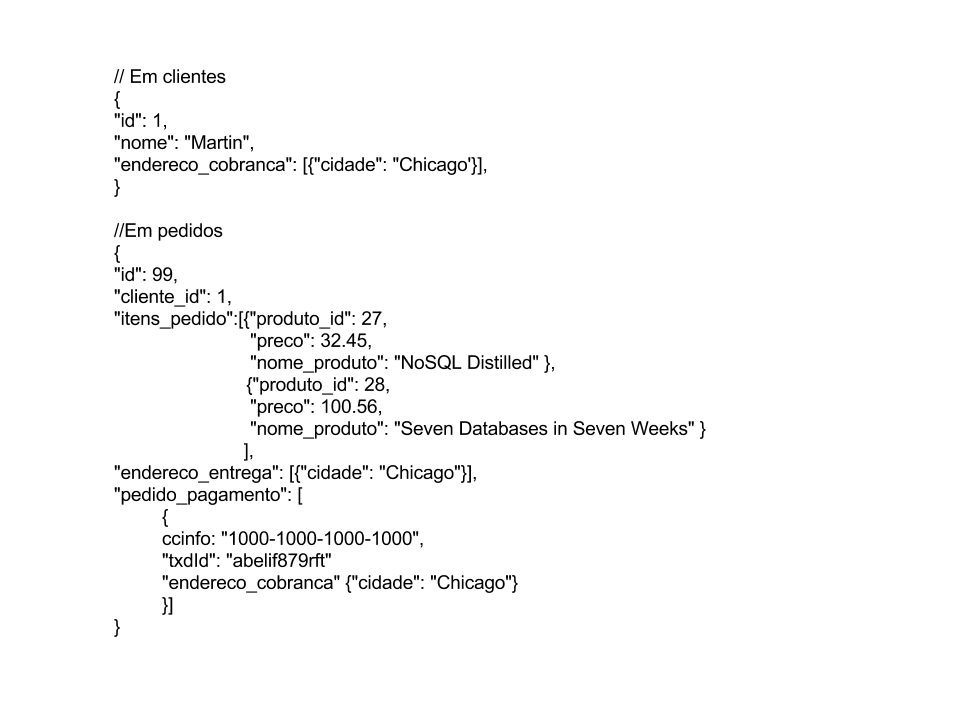
\includegraphics[width=0.8\textwidth]{./04-figuras/disposicao_json_simples.png}
    \fonte{\cite{NoSQL}}
    \label{fig:disposicao_json_simples}
\end{figure}



Observamos que as duas principais agregações são cliente e pedido. O cliente contém apenas uma lista, que é a de endereços. Já o pedido contém uma lista de itens de pedido, endereços e pagamentos. E por fim, o pagamento contém uma lista de endereços. Endereço aparece três vezes, mas ao invés de utilizar uma referência com um identificador, como no modelo relacional, o valor é copiado. Essa redundância de dados se adapta ao problema, pois, nesse caso, não queremos que o endereço em pagamento seja alterado caso o usuário altere o endereço de entrega.  Utilizando o modelo relacional, temos duas maneiras de lidar com o problema. A primeira é tratar para que não seja permitido se alterar o endereço, após ele ser vinculado à pedido ou pagamento. A segunda e mais usada, é duplicar o endereço e associá-los a pedido e pagamento. Ou seja, os dados ficam redundantes da mesma maneira. As relações entre \textit{Pedido-Cliente} e \textit{ItemPedido-Produto} funcionam da mesma maneira que o modelo relacional, um lado da relação armazena o identificador do outro lado, por exemplo, o pedido mantém o identificador do cliente relacionado.

A segunda maneira de modelar o exemplo de \textit{e-commerce} em NoSQL, seria utilizar as agregações do exemplo anterior (\textit{Pedido-Endereço}, \textit{Pedido-ItemPedido}, \textit{Pedido-Pagamento}, \textit{Cliente-Endereço}, e por fim \textit{Endereço-Pagamento}) mais a agregação entre cliente e pedido. O modelo em \ac{UML} ficaria como na \autoref{fig:diagrama_no_sql_uml_duplo} e os dados ficariam dispostos como na \autoref{fig:disposicao_json_duplo}.

\begin{figure}[H]
    \centering
    \caption{Exemplo de um diagrama \ac{UML} para utilizando agregação entre cliente e pedido}
    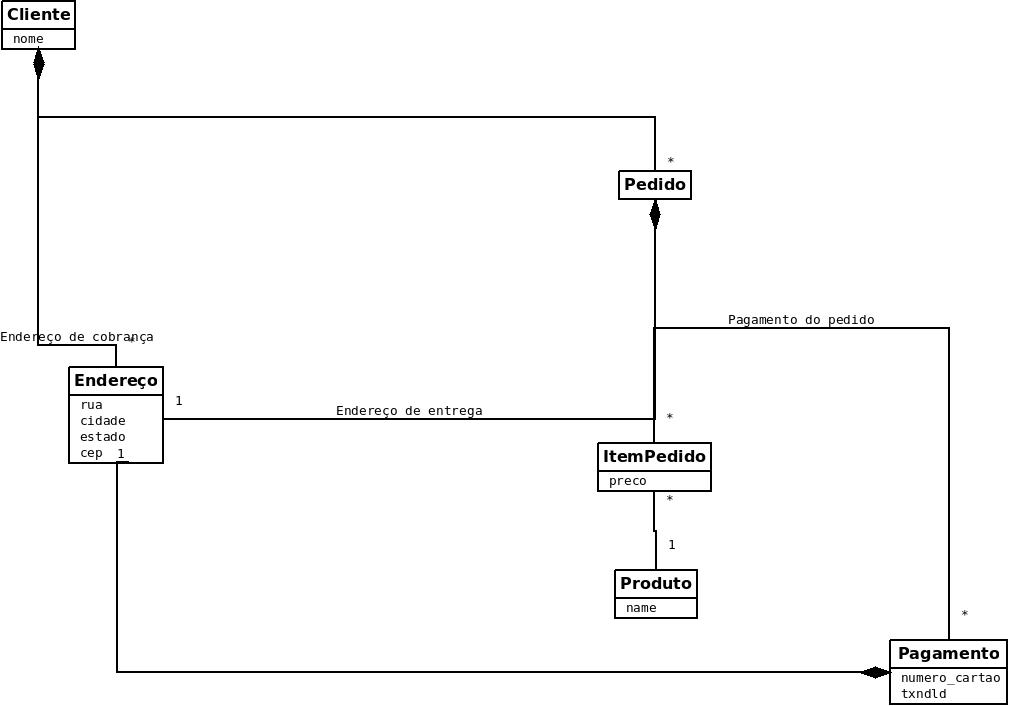
\includegraphics[width=0.8\textwidth]{./04-figuras/diagrama_no_sql_uml_duplo.jpg}
    \fonte{\cite{NoSQL}}
    \label{fig:diagrama_no_sql_uml_duplo}
\end{figure}
\begin{figure}[H]
    \centering
    \caption{Exemplo da disposição dos dados no NoSQL, utilizando agregação entre cliente e pedido}
    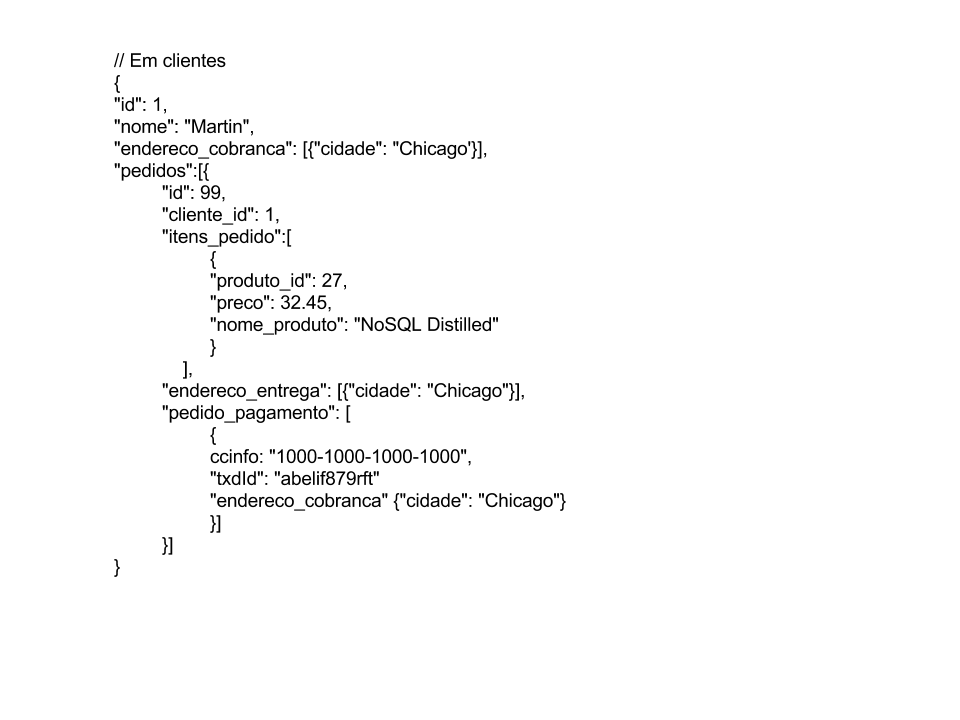
\includegraphics[width=0.8\textwidth]{./04-figuras/disposicao_json_duplo.png}
    \fonte{\cite{NoSQL}}
    \label{fig:disposicao_json_duplo}
\end{figure}

Como na maioria dos problemas de modelagem não existe a melhor solução, mas sim uma que se adapta melhor a um certo tipo de problema, devemos analisar o objetivo da aplicação para fazer uma melhor escolha.

Nesse exemplo, se for interessante para a aplicação listar o histórico dos pedidos do mês corrente, o modelo da \autoref{fig:diagrama_no_sql_uml_duplo} não é o ideal, pois será necessário entrar em cada cliente para ler os pedidos. Já utilizando o modelo da \autoref{fig:diagrama_no_sql_uml_simples}, essa busca se torna trivial \cite{NoSQL}, pois basta fazer uma busca dos pedidos que contém a data igual a do mês corrente.

Por outro lado, ao buscarmos os pedidos de um cliente, o modelo da \autoref{fig:diagrama_no_sql_uml_duplo} irá apresentar um melhor desempenho. Pois, será necessário apenas buscar o cliente que essa consulta irá trazer todos os seus pedidos. Já no modelo da \autoref{fig:diagrama_no_sql_uml_simples} será necessário percorrer pedido por pedido e comparar o identificador do cliente.

Outra razão para utilizar agregação é a facilidade proporcionada para colocar o funcionamento em ambiente distribuído. Pois, utilizando esse modelo temos a informação de quais dados devem ser manipulados juntos e se devem estar no mesmo nó do \textit{cluster}.

O modelo relacional por não tratar o conceito de agregação, ou seja, não permite campos multivalorados é chamado de \textit{aggregate-ignorant}. Apesar disso, o modelo relacional tem suas vantagens. A principal é que ao utilizar o modelo relacional, podemos analisar os dados em diversas perspectivas, já no banco de dados NoSQL algumas consultas podem ser mais complexas ou até mesmo mais lentas. Por exemplo, o modelo da \autoref{fig:diagrama_no_sql_uml_duplo} ficará mais lento para buscar o histórico de pedidos.

Outra desvantagem do NoSQL é não implementar transações do tipo \ac{ACID}. A maioria dos bancos de dados NoSQL conseguem implementar essas transações apenas sobre uma agregação como dito anteriormente. Caso seja necessário o controle dessas transações deverá ser feito no código da aplicação.

\subsection{Persistência Poliglota}
\label{subsec:polyglotpersitence}

O objeto desse trabalho são duas aplicações que utilizam dois gêneros de banco de dados: orientado a documento e chave-valor.

O gênero chave-valor funciona como uma simples tabela \textit{hash} que dado uma chave única encontrará um valor. O sistema desse banco não tem conhecimento algum sobre esse valor, logo poderá ser um texto, um objeto multivalorado, um valor binário. Qualquer tipo de informação, apenas o tamanho é limitado, dependendo do banco. Alguns exemplos de bancos desse gênero são \ac{Redis}\footnote{Sítio oficial do Redis \url{http://redis.io/}} e Riak\footnote{Sítio oficial do Riak \url{http://basho.com/riak/}}. Não existe um tratamento para consistência utilizando esse gênero, da mesma maneira que o gênero orientado a documento. Isso pode ser implementado, mas é muito custoso \cite{NoSQL}. Em relação à consistência no ambiente paralelo, cada banco implementa de uma maneira. O Riak, por exemplo, utiliza o chamado \textit{Quorums}, que é uma abordagem de consistência que elege o valor mais atual fazendo uma consulta entre os nós. Aquele valor que tiver na maioria dos nós será eleito como mais atualizado.

Como o banco não tem conhecimento da estrutura armazenada, qualquer filtro necessário deverá ser feito pela aplicação. A aplicação faz a busca no banco utilizando a chave, o banco retorna o valor referente a essa chave e em seguida, a aplicação trabalha com esse valor fazendo o filtro dos registros que deseja. Também é possível programar o tempo de expiração da chave. Essa maneira que o banco chave-valor trabalha faz com que ele se adeque bem para manter dados da sessão de um usuário, carrinhos de compra de um \textit{e-commerce}, perfil de usuários e outros. Haverá uma perda de desempenho, caso seja usado para armazenar estruturas nas quais a aplicação fará buscas comparando os dados do valor. Por exemplo, suponha que tenhamos o modelo da \autoref{fig:diagrama_no_sql_uml_duplo} para armazenar a estrutura utilizando o modelo chave-valor. Para realizar a busca de todos os pedidos do mês corrente, teremos que carregar para a aplicação todos os clientes, acessar os pedidos de cada um e verificar se a data do pedido é igual ao do mês corrente \cite{NoSQL}.

O gênero orientado a documento trabalha com o conceito de documento. O documento pode estar representado nos formatos \ac{XML}, JSON, BSON ou outros. Esses documentos são armazenados em coleções. Documentos da mesma coleção são semelhantes, mas não precisam ser idênticos. Se fizermos uma analogia, a coleção seria a tabela no modelo relacional e um documento seria uma tupla no modelo relacional. Exemplos desse gênero são MongoDB\footnote{Sítio oficial do MongoDB \url{http://www.mongodb.com/}} e CouchDB\footnote{Sítio oficial do CouchDB \url{http://couchdb.apache.org/}} \cite{NoSQL}.
Existem dois tipos de relacionamento, um que funciona semelhante ao modelo relacional que é referenciando um documento de uma coleção pelo identificador, análogo a chave estrangeira no modelo relacional. Outro tipo é embutir documentos dentro de um documento, ou seja, agregação. Consistência existe apenas para os objetos da agregação, como relatado anteriormente. Quando distribuído, o MongoDB pode trabalhar com uma série de políticas de como irá se comportar no ambiente paralelo, que são configuráveis. Esse gênero não implementa transações\footnote{Operações de inserir, atualizar ou deletar com a opção de emitir o \textit{commit} ou \textit{rollback}}. O MongoDB permite que sejam feitas consultas com filtros e a linguagem utilizada é o JavaScript. Consultas mais complexas que utilizam os documentos embutidos em outros documentos são realizadas com \textit{MapReduce} \cite{NoSQL}. Por exemplo, se modelarmos esse banco com o modelo da \autoref{fig:diagrama_no_sql_uml_duplo} para fazer a busca dos pedidos do mês corrente, diferente do \ac{Redis}, o banco é capaz de fazer esse filtro e retornar apenas os pedidos que têm a data igual a do mês corrente. Para isso ele utiliza \textit{MapReduce}.

Diferentes bancos de dados foram desenhados para resolver diferentes problemas \cite{NoSQL}. Conseguir identificar diferentes problemas de armazenamento, representação ou escalabilidade dentro de uma aplicação pode ser um indicativo de que mais de um banco de dados deve ser utilizado. Da mesma maneira que diferentes paradigmas de linguagem de programação são utilizados em um desenvolvimento Web, diferentes gêneros de banco de dados podem ser usados em uma mesma aplicação \cite{multiparadigma}. A persistência poliglota consiste em que uma aplicação utiliza mais de um banco de dados.

Neste trabalho fizemos a implementação de dois sistemas similares ao Twitter, sendo que um utiliza a persistência monoglota e outro a persistência poliglota. No próximo capítulo, está descrita a implementação dos dois sistemas.


